\documentclass[letterpaper,11pt,leqno]{article}
\usepackage{paper}
\usepackage{tikz}
\usepackage{multirow}
\usepackage{dirtytalk}
\usepackage{float}
\usetikzlibrary{arrows,positioning,shapes}
\bibliographystyle{bibliography}

% Enter paper title to populate the PDF metadata:
\hypersetup{pdftitle={Minimalist LaTeX Template for Academic Papers}}

% Enter BibTeX file with references:
\newcommand{\bib}{bibliography.bib}

% Enter PDF file with figures:
\newcommand{\pdf}{figures.pdf}

\begin{document}

% Enter title:
\title{Individual violin sound identification using audio features and machine learning}

% Enter authors:
\author{Hugo Pauget Ballesteros, Claudia Fritz, Philippe Lalitte
%
% Enter affiliations and acknowledgements:
\thanks{First Author: First University. Second Author: Second University. We thank colleagues for helpful comments and discussions. This work was supported by a grant [grant number]; another grant [grant number]; and a foundation.}}

% Enter date:
\date{June 2024}   

\begin{titlepage}
\maketitle

% Enter abstract:
Few articles have addressed the issue of identifying individual instruments of the same type from their recordings. In this paper, we explore violin sound identification using audio features and machine learning algorithms. A review and a comparison between different approaches is made, which allow

\end{titlepage}

% Enter main text:
\section{Introduction}\label{s:introduction}
 
Musical instruments classification is a Musical Information Retrieval (MIR) task which consists of determining the instruments present in a recording. This topic has been extensively studied in the literature, and for monophonic recordings (containing only one instrument), state-of-the-art models reach often almost $100\%$. However, few articles have addressed the issue of identifying individual instruments of the same type, let alone from the violin familiy specifically.

In \cite{lukasikLongTermCepstral2010b}, 

The goal of this paper is to review and compare different ways of tackling this task, from data collection to data processing. Guidelines regarding recording sessions are discussed and a Long-Time version of MFCCs is introduced.

This paper is structured as follows: Section \ref{s:methodology} presents the methodology of our experiment, describing data collection, features extraction, data exploration and finally classification using machine learning methods. Results of the experiments are discussed in Section \ref{s:results}. Finally, conlusions are drawn in Section \ref*{s:conclusions}, which also outlines possible future developments. 

\section{Methodology}\label{s:methodology}

\subsection{Dataset}

During the Bilbao Project, thirteen violins were built in order to relate their material and geometrical characteristics with their tonal quality \citep{fritzBilbaoProjectSearching2021}. These violins have been played in 2019 by twenty-three professional violinists, each of them having recorded a scale on each violin and a short musical excerpt on a violin of their choice. The recordings were made under the same conditions in a large rehearsal room at the Bilbao conservatory, keeping the distance between the player and the microphone constant. Our dataset thus consists of $13 \times 23$ scales plus $1 \times 23$ musical excerpts.

\begin{figure}[h]
	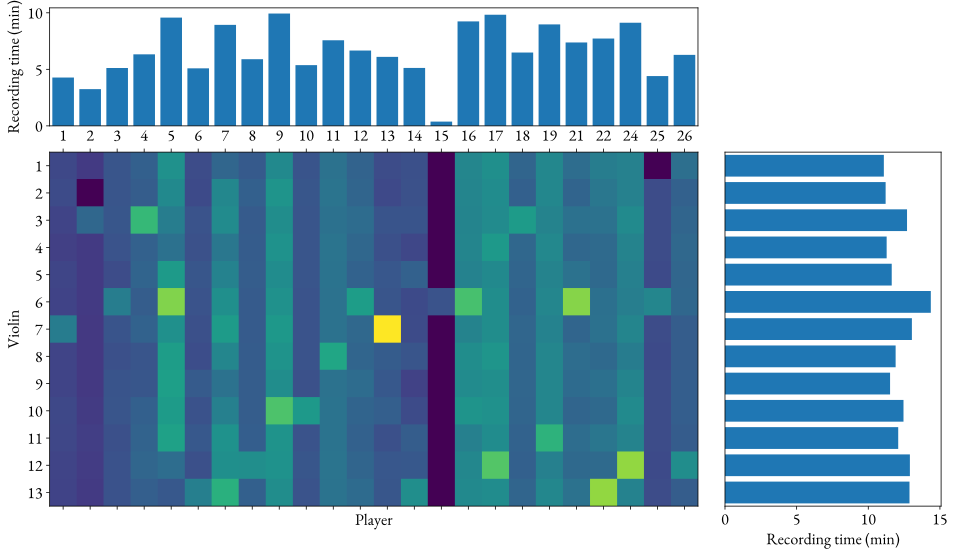
\includegraphics[width=0.8\textwidth]{../figures/class_weights.png}
	\caption{Recording time available with respect to players and with respect to violins}
\end{figure}

Six of those thirteen Bilbao violins (violins number 1, 4, 5, 9, 11 and 13) were brought to the 2024 Villfavard Workshop and were recorded again. They were played freely by four new players in a small room, under rather different conditions than during the 2019 recordings.

\begin{figure}[h]
	\includegraphics[width=0.8\textwidth]{../figures/class_weights_2024.png}
	\caption{Recording time available with respect to players and with respect to violins}
\end{figure}

\subsection{Features}

The following features have been compared for the classification task :

\subsubsection{Long Time Average Spectra (LTAS)}{

The Long Time Average Spectra (LTAS) of a recording is obtained by dividing the input signal into overlapping segments, then calculating the windowed DFT of each segment and finally averaging the power of those DFTs :

\begin{figure}[!h]
	\begin{tikzpicture}
		% \usetikzlibrary{arrows,positioning,shapes}
		\tikzstyle{entry} = [draw=none, text width=3em, text centered, minimum height=3em]
		\tikzstyle{block} = [rectangle, draw, text width=4em, text centered, rounded corners, minimum height=3em]
		\tikzstyle{arrow} = [draw, -latex']
		\node [entry] (signal) {Signal};
		\node [block, right=of signal] (window) {Window};
		\node [block, right=of window] (dft) {DFT};
		\node [block, right=of dft] (power) {$|\cdot|^2$};
		\node [block, right=of power] (average) {Average};
		\node [entry, right=of average] (ltas) {LTAS};

		\path[draw,->] (signal) edge (window);
		\path[draw,->] (window) edge (dft);
		\path[draw,->] (dft) edge (power);
		\path[draw,->] (power) edge (average);
		\path[draw,->] (average) edge (ltas);
	\end{tikzpicture}
\end{figure}

LTAS has been used in \cite{buenCOMPARINGSOUNDGOLDEN2005} in order to compare the tonal quality of violins. More specifically, the sound of old Italians violins (Stradivari/Guarneri) and modern violins has been compared. The author concludes that differences between these two groups can be shown using LTAS

\begin{figure}[h]
	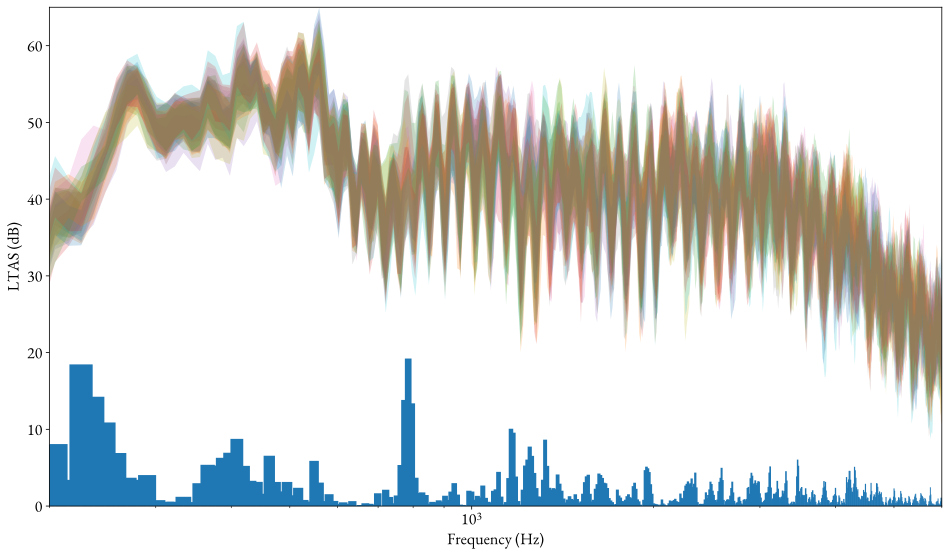
\includegraphics[width=0.8\textwidth]{../figures/ltas.png}
	\caption{Standard Deviation of the LTAS of the 13 violins with respect to players}
\end{figure}
}

\subsubsection{Mel-Frenquency Cepstral Coefficients (MFCC)}{
	MFCCs are obtained by mapping the frequencies of a spectrum onto a nonlinear mel-scale (a perceptual scale of pitches judged by listeners to be equal in distance from one another), taking the log, and then compute the DCT of the result. Here, instead of calculating the MFCCs on overlapping segments, we use a LTAS as our spectra as we want features with a long-term meaning :

	\begin{figure}[!h]
		\begin{tikzpicture}
			% \usetikzlibrary{arrows,positioning,shapes}
			\tikzstyle{entry} = [draw=none, text width=3em, text centered, minimum height=3em]
			\tikzstyle{block} = [rectangle, draw, text width=3em, text centered, rounded corners, minimum height=3em]
			\tikzstyle{arrow} = [draw, -latex']
			
			\node [entry] (signal) {Signal};
			\node [block, right=of signal] (ltas) {LTAS};
			\node [block, right=of ltas] (mel) {Mel \\ Filter};
			\node [block, right=of mel] (log) {Log};
			\node [block, right=of log] (dct) {DCT};
			\node [entry, right=of dct] (mfcc) {MFCC};

			\path[draw,->] (signal) edge (ltas);
			\path[draw,->] (ltas) edge (mel);
			\path[draw,->] (mel) edge (log);
			\path[draw,->] (log) edge (dct);
			\path[draw,->] (dct) edge (mfcc);
		\end{tikzpicture}
	\end{figure}

	MFCC are a set of features that has been extensively used for Automatic Speaker Recognition and for Instruments Classification.

	\begin{figure}[!h]
		
\includegraphics[width=0.8\textwidth]{../figures/ltcc.png}
		\caption{Standard Deviation of the LTAS of the 13 violins with respect to players}
	\end{figure}
}

\subsubsection{Long-Term Cepstral Coefficients (LTCC)}{
	LTCC have been introduced in \cite{lukasikLongTermCepstral2010b} for Indivudial Instrument Identification. Their calculation is similar to that of MFCCs, except that a Mel-filterbank is not applied and that the final step is given by an Inverse Discrete Fourier Transform. 

	\begin{figure}[!h]
		\begin{tikzpicture}
			\tikzstyle{entry} = [draw=none, text width=3em, text centered, minimum height=3em]
			\tikzstyle{block} = [rectangle, draw, text width=3em, text centered, rounded corners, minimum height=3em]
			\tikzstyle{arrow} = [draw, -latex']
			\node [entry] (signal) {Signal};
			\node [block, right=of signal] (ltas) {LTAS};
			\node [block, right=of ltas] (log) {Log};
			\node [block, right=of log] (idft) {iDFT};
			\node [entry, right=of idft] (ltcc) {LTCC};

			\path[draw,->] (signal) edge (ltas);
			\path[draw,->] (ltas) edge (log);
			\path[draw,->] (log) edge (idft);
			\path[draw,->] (idft) edge (ltcc);
		\end{tikzpicture}
	\end{figure}

	\begin{figure}[!h]
		
\includegraphics[width=0.8\textwidth]{../figures/ltcc.png}
		\caption{Standard Deviation of the LTAS of the 13 violins with respect to players}
	\end{figure}
}

\subsection{Data exploration}

\subsubsection{Variability of LTAS}

\subsubsection{Feature selection}

\subsection{Classification}

We compare the results of three popular classification algorithms : K-Nearest Neighbours, Support Vector Machines and Multilayer Perceptron. These three classifiers use different learning strategies and thus will give different results on our data.

\subsubsection{K-Nearest Neighbours}

K-Nearest Neighbours is a method that finds the closest training points to a new test point and predicts its label from them. Since the prediction is made directly from the training data, this method is non-parametric (or non-generalizing), which is an advantage when the decision boundary is irregular.


\subsubsection{Support Vector Machines}

Support Vector Machines is a supervised learning method using for classification. It works by finding an optimal hyperplane that maximizes the distance between each class in the training data. This algorithm is computationally expensive but generally has good generalisation properties.

\subsubsection{Multilayer Perceptron}

Multilayer perceptron is a supervised learning method that learns a function $f : \mathbb{R}^n \to \mathbb{R}^o$ using training data. To do so, it uses layers of neurons as in Figure \ref{f:mlp}. Each neuron transforms the result from the previous layer by forming a weighted linear summation $w_0 + w_1 x_1 + \dots + w_n x_n$ followed by a non-linear activation function.

\begin{figure}[H]
	\includegraphics[width=0.5\textwidth]{../figures/multilayerperceptron_network.png}
	\caption{Multilayer Perceptron}
	\label{f:mlp}
\end{figure}

This method has demonstrated effectiveness in various domains, as the non-linear activation functions can model complex relationships in data while hidden layers can learn hierarchical representations from input data. However, MLPs are prone to overfitting, especially on small datasets.

\section{Results}\label{s:results}

In this section we present the results of the classification task performed on different subsets of the dataset. We compare the results of each feature paired with each classifier. The results showed below are the one after fine-tuning the hyper-parameters, which can be hyper-parameters in the computation of the feature (sample rate, sample duration, ...) or hyper-paramters of the classification algorithm ($k$ for K-NN, for instance).

\begin{table}[H]
\caption{Results using scales as training data and muscial excertps as test data}  
\centering
	\begin{tabular}{c c c c}
		\textbf{Method} & \textbf{Feature} & \textbf{Train} & \textbf{Test} \\
		\hline\hline
		\multirow{3}{3em}{K-NN} & LTAS & 100\% & 37\% \\
		& LTCC & 100\% & 100\% \\
		& MFCC & 100\% & 100\% \\
		\hline
		\multirow{3}{3em}{SVM} & LTAS & 100\% & 37\% \\
		& LTCC & 100\% & 100\% \\
		& MFCC & 100\% & 100\% \\
		\hline
		\multirow{3}{3em}{MLP} & LTAS & 100\% & 37\% \\
		& LTCC & 100\% & 100\% \\
		& MFCC & 100\% & 100\% \\
		\hline
	\end{tabular}
\end{table}

\begin{table}[H]
	\caption{Results using cross-validation on the entire dataset}  
	\centering
		\begin{tabular}{c c c c}
			\textbf{Method} & \textbf{Feature} & \textbf{Train} & \textbf{Test} \\
			\hline\hline
			\multirow{3}{3em}{K-NN} & LTAS & 100\% & 37\% \\
			& LTCC & 100\% & 100\% \\
			& MFCC & 100\% & 100\% \\
			\hline
			\multirow{3}{3em}{SVM} & LTAS & 100\% & 37\% \\
			& LTCC & 100\% & 100\% \\
			& MFCC & 100\% & 100\% \\
			\hline
			\multirow{3}{3em}{MLP} & LTAS & 100\% & 37\% \\
			& LTCC & 100\% & 100\% \\
			& MFCC & 100\% & 100\% \\
			\hline
		\end{tabular}
	\end{table}

\section{Conclusions}\label{s:conclusions}



\bibliography{\bib}

\end{document}